
\chapter{Organization of the Implementation}

To organize our implementation phase, we decided first to look deeper inside the project and try to extract problems and divide them into separate milestones. We knew that we want to use top-down approach for our implementation phase. Even before implementation phase began, we knew that we want to get into smaller groups (2-3 people) and work separately on \gls{frontend} and \gls{backend}. Then, we could meet all together in person once every 2 days to discuss our progress, ask for advice or opinion on some topics and new changes to the design. For our online communication, be it sharing links, organization moments or online meetings we used our \gls{discord} server, that we had since our draft statement phase.

To have a better overview on the current progress and to track problems, we had to modify our GitLab repository:
\begin{itemize}
    \item First, we created new milestones:
          \begin{description}
              \item[Backend Core] All issues related to the armarest package and general structure of the backend.
              \item[Backend: Logger impl] All issues related to the implementation of the logger in the backend.
              \item[Backend: KinematicUnit impl] All issues related to the implementation of the KinematicUnit in the backend.
              \item[Backend: Remote Impl] All issues related to the implementation of the RemoteGUI in the backend.
              \item[Backend: Emergency Stop Service] All issues related to the implementation of the Emergency Stop Service in the backend.
              \item[Command-Line Interface] All issues related to the implementation of the \gls{cli}.
              \item[Frontend impl] All issues related to the implementation of the different parts and pages in the frontend.
              \item[Report] Writing an implementation report.
          \end{description}
    \item Then we established around 30 different implementation issues, be it for example \textit{Implement the EmergencyStopCore} or \textit{Implement Navigation Bar in frontend}, labeled them by milestones and tags (bug, small issues, large issue...). We knew that we couldn't possibly establish all issues that we have to deal with, but it was a good starting point.
    \item We assigned current established issues to everyone, according to our preferences, knowledge and experience.
\end{itemize}


During the process, we found new issues and divided existing ones. This is a simplified overview of our workflow:
\begin{enumerate}
    \item Select an issue assigned to us.
    \item Create a new merge request from the \textit{main} branch (we had a strict policy about not being able to change \textit{main} branch directly).
    \item Work on this issue remotely and push changes to the branch.
    \item Select another member of team to review a merge request.
    \item If another member of team approves it, the new branch is merged into the \textit{main} branch
\end{enumerate}
At the end of the phase we had around 60 different issues.

\begin{figure}[h]
    \caption{Example of issues in the GitLab}
    \centering
    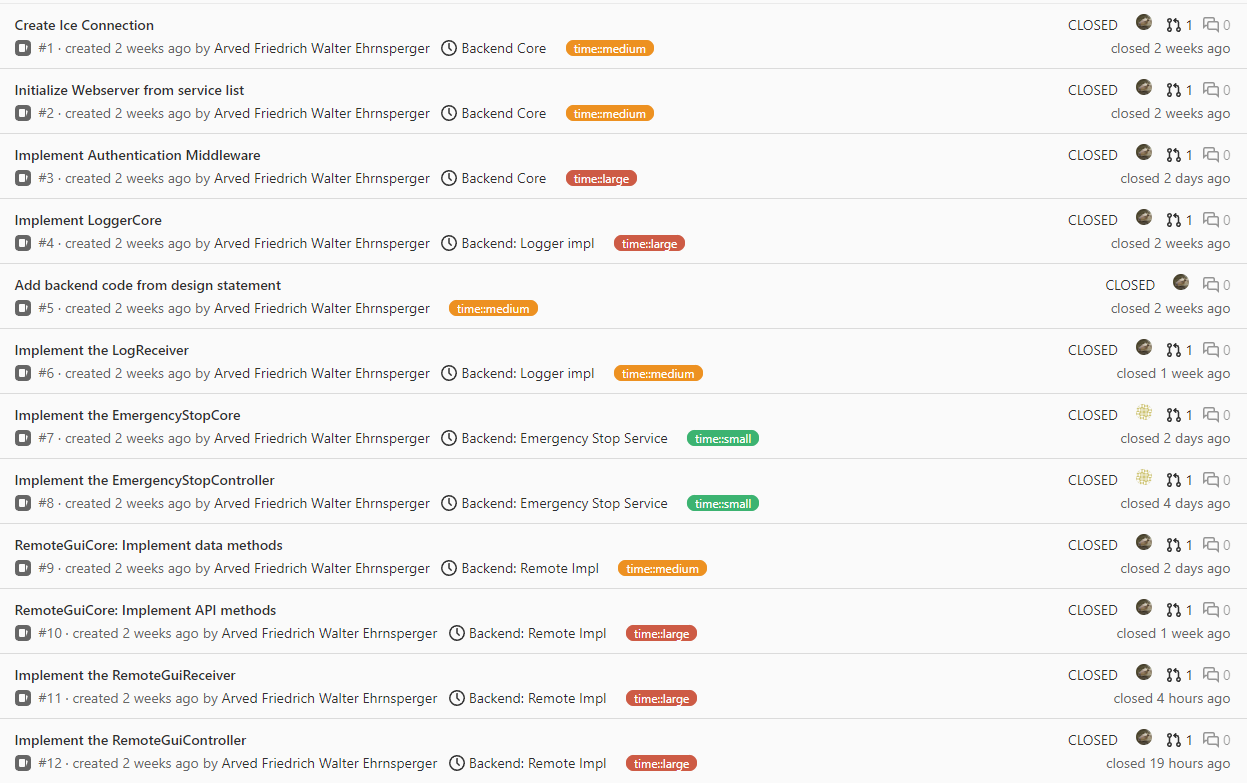
\includegraphics[scale=0.65]{images/issues.png}
\end{figure}
